%!TEX ROOT = thesis.tex
\chapter{Symbol Error Rate (SER) for 16-QAM Modulation} \label{appendC}

\addcontentsline{toc}{chapter}{APPENDIX C: Symbol Error Rate (SER) for 16-QAM Modulation}
% % % % % % % % % % % % % % % % % % % % % % % % %
\begin{figure}[!h]
%\captionsetup{list=no}
%\stepcounter{figure}
\centering
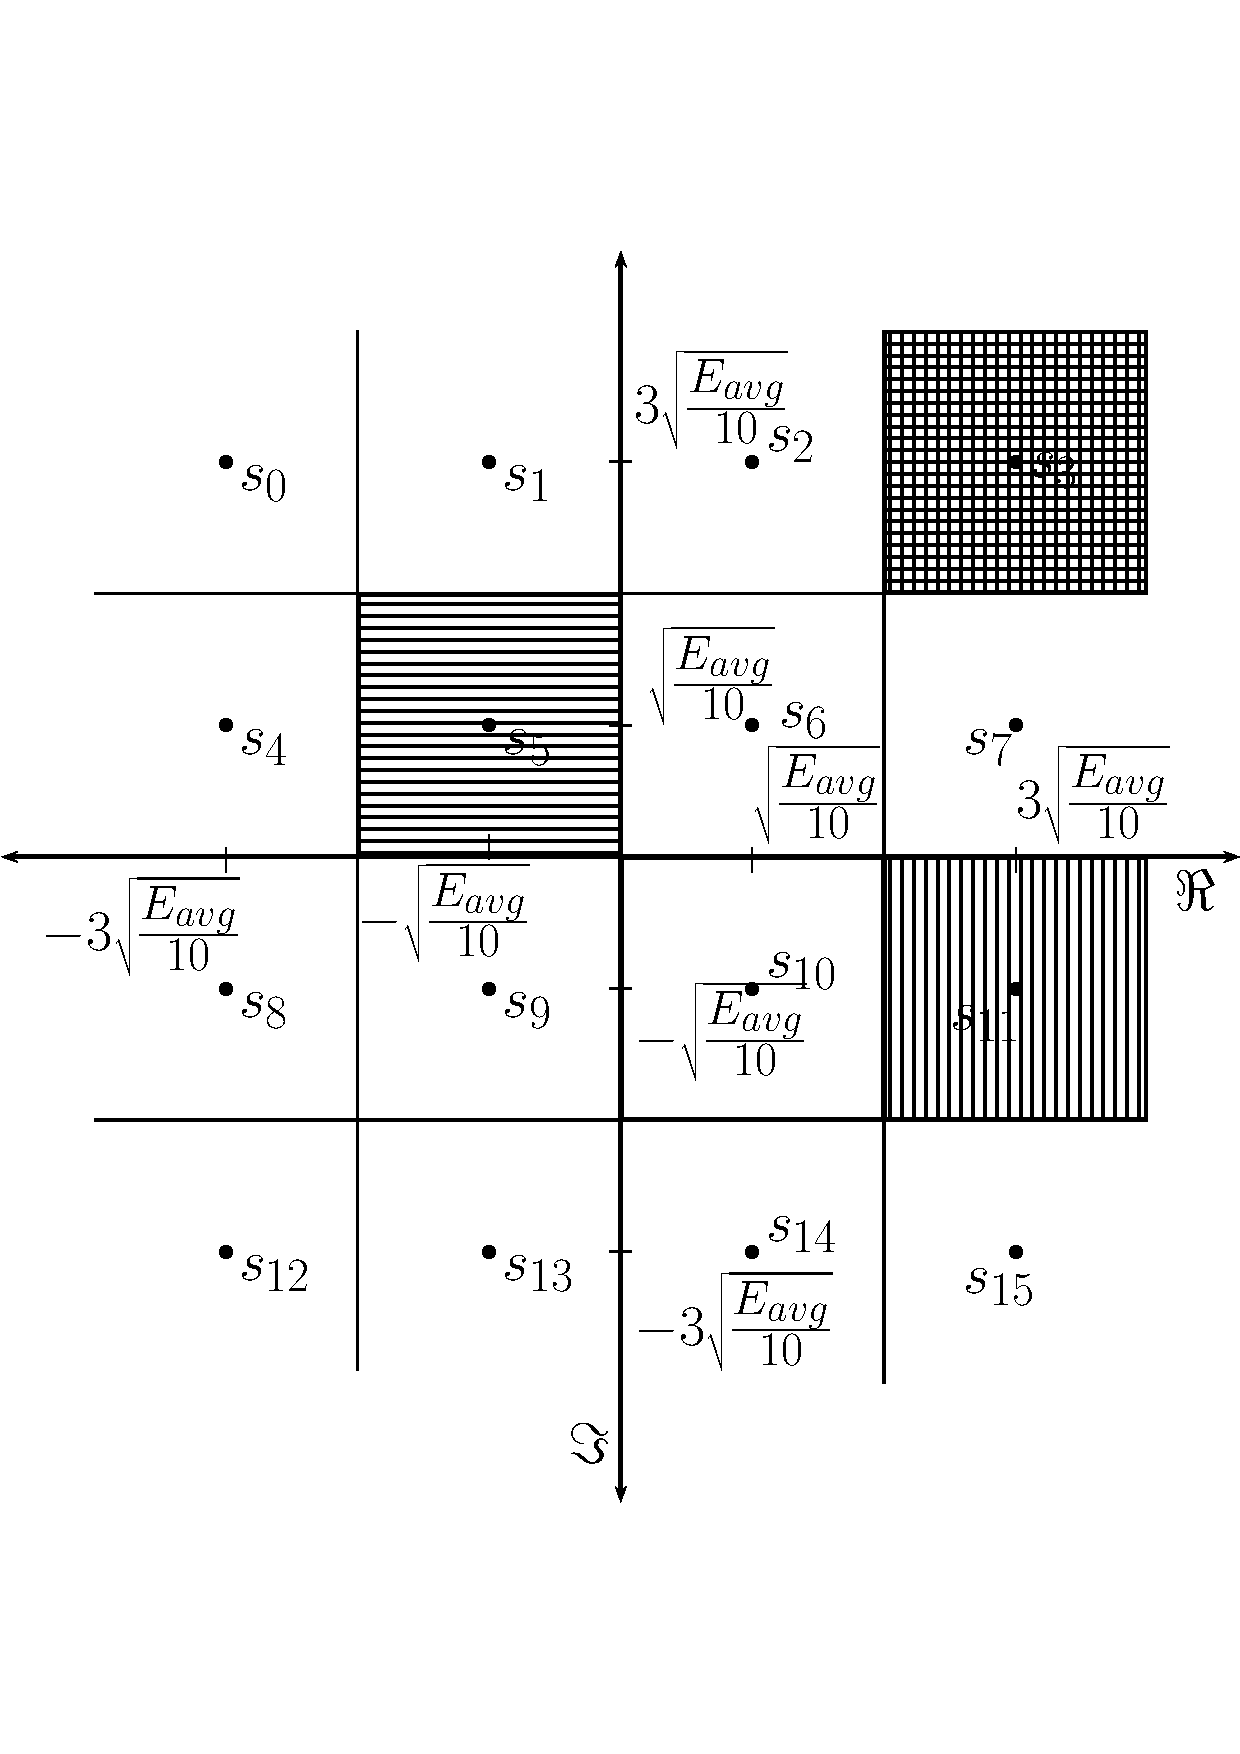
\includegraphics[width=0.6\textwidth]{./append3/SER16QAM}
%\legend{\figurename~\thefigure:~16-QAM constellation.}
\caption{16-QAM constellation.}
\label{figIII:QAM_const}
\end{figure}
The average signal energy is given by:
\begin{equation}\label{eqnIII:averagepower}
	E_{avg}=\sum\limits_{m=1}^{M}p_mE_m
\end{equation}
where $ pm $ is the message probability. $ E_m $ is symbol energy for message $ m $, $ M $ is the modulation order, for 16-QAM, $M=16  $. If all symbols have the same probability (e.g equiprobable message) the equation~\eqref{eqnIII:averagepower} becomes:
  \begin{equation}
  E_{avg}=\dfrac{5}{2}d^2
  \end{equation}
  where $ d $ is the minimum distance between two consecutive constellations. In terms of average energy per bit $ E_{bavg} $:
  \begin{equation}
  E_{bavg}=\dfrac{E_{avg}}{\log_2M}
  \end{equation}
  \begin{equation}
  \dfrac{d}{2}= \sqrt{\dfrac{E_{avg}}{10}}
  \end{equation}
  
\noindent The alphabets of a 16-QAM modulation scheme are:\\ 
$ \alpha=\{\pm 1 + \pm 1j, \pm + \pm 3j, \pm + \pm 3j, \pm + \pm 1j\} $
\par The conditional probability distribution function (PDF) of $ y $ given $ s_5 $ was transmitted:
	\begin{align}
	f(y/s_5)&=\dfrac{1}{\sqrt{\pi N_0}}e^{\frac{{-\big ( y-\sqrt{\frac{E_{avg}}{10}}\big )}^2}{N_0}}
	\end{align}
	
	%\begin{small}
		From figure~\ref{figIII:QAM_const}, symbol $ s_{5} $ is detected correctly if $ y $ falls in the horizontally shaded area, i.e.,
	\begin{align*}
	f(c|s_5)=&f \Bigg(\Re\{y\} \le 0,\Re\{y\}>-2\sqrt{\dfrac{E_{avg}}{10}} \Big|s_5 \Bigg ).\\
	&f\Bigg (\Im\{y\}>0,\Im\{y\}\leq 2\sqrt{\dfrac{E_{avg}}{10}} \Big| s_5 \Bigg )
	\end{align*}
		Using the relation:
	  \begin{equation}
	f(c|s_5)=\Bigg[ 1-\text{erfc}\Bigg( \sqrt{\dfrac{E_{avg}}{10N_0}} \Bigg)\Bigg]\Bigg[ 1-\text{erfc}\Bigg( \sqrt{\dfrac{E_{avg}}{10N_0}} \Bigg)\Bigg]
	\end{equation}
		The probability of error for $ s_5 $ is:
	\begin{align}
	f(e|s_5)&=1-\Bigg[ 1-\text{erfc}\Bigg( \sqrt{\dfrac{E_{avg}}{10N_0}} \Bigg)\Bigg]^2\\
	&\approx 2\text{erfc}\Bigg( \sqrt{\dfrac{E_{avg}}{10N_0}} \Bigg)
	\end{align}
	
	
		The conditional probability distribution function (PDF) of $ y $ given $ s_3 $ was transmitted is:
		\begin{align}
		f(y/s_3)&=\dfrac{1}{\sqrt{\pi N_0}}e^{\frac{{-\big ( y-\sqrt{\frac{E_{avg}}{10}}\big )}^2}{N_0}}
		\end{align}
		
		From Figure~6, symbol $ s_{3} $ is detected correctly if $ y $ falls in the crossed shaded area, i.e.,
		\begin{align*}
		f(c|s_3)=f \Bigg(\Re\{y\}>2\sqrt{\dfrac{E_{avg}}{10}} \Big|s_3 \Bigg )f\Bigg (\Im\{y\}> 2\sqrt{\dfrac{E_{avg}}{10}} \Big| s_3 \Bigg )
		\end{align*}
		%\end{small}
		Using the relation:
		\begin{equation}
		f(c|s_3)=\Bigg[ 1-\dfrac{1}{2}\text{erfc}\Bigg( \sqrt{\dfrac{E_{avg}}{10N_0}} \Bigg)\Bigg]\Bigg[ 1-\dfrac{1}{2}\text{erfc}\Bigg( \sqrt{\dfrac{E_{avg}}{10N_0}} \Bigg)\Bigg]
		\end{equation}
		The probability of error for $ s_3 $ is:
		\begin{align}
		f(e|s_3)&=1-\Bigg[ 1-\dfrac{1}{2}\text{erfc}\Bigg( \sqrt{\dfrac{E_{avg}}{10N_0}} \Bigg)\Bigg]^2\\
		&\approx \text{erfc}\Bigg( \sqrt{\dfrac{E_{avg}}{10N_0}} \Bigg)
		\end{align}
		
		
				The conditional probability distribution function (PDF) of $ y $ given $ s_{11} $ was transmitted:
				\begin{align}
				f(y/s_{11})&=\dfrac{1}{\sqrt{\pi N_0}}e^{\frac{{-\big ( y-\sqrt{\frac{E_{avg}}{10}}\big )}^2}{N_0}}
				\end{align}
				%\begin{small}
				From figure~\ref{figIII:QAM_const}, symbol $ s_{11} $ is detected correctly if $ y $ falls in the vertically shaded area, i.e.,
				\begin{align*}
				f(c|s_{11})=f \Bigg(\Re\{y\}>2\sqrt{\dfrac{E_{avg}}{10}} \Big|s_{11} \Bigg )f\Bigg (\Im\{y\}\leq 0,\Im\{y\}> -2\sqrt{\dfrac{E_{avg}}{10}} \Big| s_{11} \Bigg )
				\end{align*}
				%\end{small}
				Using the above two cases as reference
				\begin{equation}
				f(c|s_{11})=\Bigg[ 1-\dfrac{1}{2}\text{erfc}\Bigg( \sqrt{\dfrac{E_{avg}}{10N_0}} \Bigg)\Bigg]\Bigg[ 1-\text{erfc}\Bigg( \sqrt{\dfrac{E_{avg}}{10N_0}} \Bigg)\Bigg]
				\end{equation}
				The probability of error of $ s_{11} $ :
				\begin{align}
				f(e|s_{11})&=1-\Bigg[ 1-\dfrac{1}{2}\text{erfc}\Bigg( \sqrt{\dfrac{E_{avg}}{10N_0}} \Bigg)\Bigg]\Bigg[ 1-\text{erfc}\Bigg( \sqrt{\dfrac{E_{avg}}{10N_0}} \Bigg)\Bigg]\\
				&\approx \dfrac{3}{2}\text{erfc}\Bigg( \sqrt{\dfrac{E_{avg}}{10N_0}} \Bigg)
				\end{align}
				The total symbol probability of 16-QAM:
				  \begin{align}
				  P_{e,16QAM}\approx \dfrac{3}{2}\text{erfc}\Bigg( \sqrt{\dfrac{E_{avg}}{10N_0}} \Bigg)				
				\end{align}
